%!TEX root = ../thesis.tex
\renewcommand\thechapter{A}
\chapter{Appendix A: Gantt Diagrams}
\label{AppendixA}

This Appendix contains the ...

\section{Ripartizione ore 1}

\begin{tabularx}{\textwidth}{c|X}
	\centering\textbf{Durata in ore} & \multicolumn{1}{c}{\textbf{Descrizione dell'attività}}\\\hline
	\textbf{70}&\textbf{Formazione sulle tecnologie}\\\hline
	\textbf{20}&\textbf{Analisi dei requisiti}\\\hline
	\textbf{40}&\textbf{Setup dell'infrastruttura}\\\hline
	\textbf{50}&\textbf{Configurazione dei servizi}\\\hline
	\textbf{60}&\textbf{Integrazione}\\\hline
	\textbf{100}&\textbf{Test}\\\hline
	\textbf{20}&\textbf{Stesura manuali}\\\hline
	\textbf{40}&\textbf{Migrazione}\\\hline
	\textbf{10}&\textbf{Collaudo Finale}\\\hline
	\textbf{Totale ore}&\multicolumn{1}{c}{\textbf{410}} \\	
\end{tabularx}


\section{Ripartizione ore 2}

\begin{tabularx}{\textwidth}{c|X}
	\centering\textbf{Durata in ore} & \multicolumn{1}{c}{\textbf{Descrizione dell'attività}}\\\hline
	\textbf{70}&\textbf{Formazione sulle tecnologie}\\\hline
	\textbf{20}&\textbf{Analisi dei requisiti}\\\hline
	\textbf{41}&\textbf{Setup dell'infrastruttura}\\\hline
	\textbf{50}&\textbf{Configurazione dei servizi}\\\hline
	\textbf{60}&\textbf{Integrazione}\\\hline
	\textbf{120}&\textbf{Test}\\\hline
	\textbf{22}&\textbf{Stesura manuali}\\\hline
	\textbf{15}&\textbf{Collaudo Finale}\\\hline
	\textbf{Totale ore}&\multicolumn{1}{c}{\textbf{410}} \\	
\end{tabularx}

\begin{landscape}
	\vspace*{\fill}
	\section{GANTT 1}
	\label{gantt_1}
	\begin{figure}[H]
		\centering
		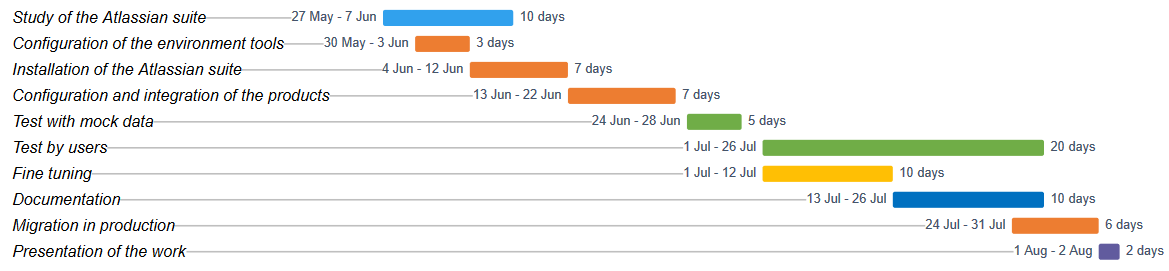
\includegraphics[width=22cm]{resources/work_plan_gantt}\\
		\caption{Gantt diagram contained in the ``\textit{Piano di Lavoro}'' document}
	\end{figure}
	\vspace*{\fill}
\end{landscape}
\newpage
\begin{landscape}
	\vspace*{\fill}
	\section{GANTT 2}
	\label{gantt_2}
	\begin{figure}[H]
		\centering
		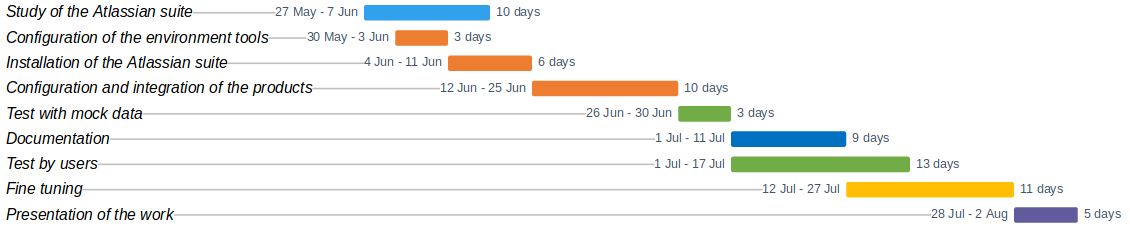
\includegraphics[width=22cm]{resources/revised_gantt}\\
		\caption{Gantt diagram contained in the ``\textit{Piano di Lavoro}'' document}
	\end{figure}
	\vspace*{\fill}
\end{landscape}